\documentclass[es]{uc3mreport}


\usepackage[utf8]{inputenc}
\usepackage[T1]{fontenc}

\usepackage{import}  % import TeX files
\usepackage{graphicx}



% general config

\graphicspath{{img/}}  % Images folder
\addbibresource{references.bib}  % bibliography file

\degree{Grado en Ingeniería Informática}
\subject{Visión Artificial}
% \shortsubject{LTX}  % optional
\academicyear{2024-2025}
\group{85}
\author{
    César López Mantecón  -- 100472092\\
    Álvaro Guerrero Espinosa -- 100472294\\
    José Antonio Verde Jiménez -- 100069420}
% \team{Equipo 69}  % optional

\shortauthor{\abbreviateauthor{César}{L.M.}, \abbreviateauthor{Álvaro}{G.E.} y \abbreviateauthor{José A.}{V.J.}}
\lab{Práctica 2}
\title{Inversión de Neural Style}
% \shorttitle{La mejor memoria de la historia}  % optional
\professor{Fernando Díaz de María\\Leire Paz Arbaizar}  % optional


% report

\begin{document}
    \makecover

%    \tableofcontents
    % \listoffigures
    % \listoftables

    % contenidos
    \begin{report}
        \section{Propuesta}
        El objetivo de este proyecto es el estudio de la capacidad de la red
        para deshacer la transformación de estilo aplicando la imagen de
            contenido original como imagen de estilo a una previamente
            transformada. Es decir, se ha transformado una imagen aplicando un
            estilo y se ha tratado de recuperar la imagen original aplicando
            esta última como estilo.

        La imagen empleada para la primera transformación será la que se muestra en la figura~\ref{original}.


        \section{Metodología}
        Para estudiar distintintas alternativas, cada uno de los miembros del
        equipo ha trabajando por separado y con un estilo diferente. Con esto, se ha buscado de forma
        independiente una solución al problema planteado. A continuación se
        expone qué alternativas ha explorado cada integrante.

            

            \subsection{César López Mantecón}
            Se ha explorado la propuesta variando el número de capas
            convolucionales y limitando la imagen a 128 píxeles. Por último, se
            ha tratado de recuperar una imagen lo más parecida a la original
            empleando otra parecida como imagen de estilo.

            La imagen de estilo utilizada para generar la primera
            transformación (la que se tratará de deshacer) es una pintura del
            artista catalán Joan Miró (figura~\ref{joan-miro}).

            La imagen intermedia, resultado de aplicar la
            imagen~\ref{joan-miro} como estilo a la original se puede ver
            en~\ref{intermedio-clm}.

            \subsection{Álvaro Guerrero Espinosa}
            Se ha explorado la propuesta variando utilizando imágenes de 128
            píxeles y variando el peso del estilo relativo al peso del
            contenido. Se ha intentado recuperar una imagen lo más parecida a la
            original, pero intentando obtener al mismo tiempo una imagen intermedia
            que represente correctamente el contenido y el estilo de las imágenes
            utilizadas. Esto se decidió para evitar la solución trivial en la que se
            establece un peso de estilo muy bajo que hace que todas las imágenes
            sean iguales a la de contenido.

            La imagen de estilo utilizada para generar la primera
            transformación (la que se tratará de deshacer) es una imagen
            promocional de un videojuego (figura~\ref{tm}).

            La imagen intermedia, resultado de aplicar la
            imagen~\ref{tm} como estilo a la original se puede ver
            en~\ref{intermedio-age}.

            \subsection{José Antonio Verde Jiménez}
            Se ha explorado la propuesta utilizando imágenes tanto de 128 como
            512 píxeles en CPU como en GPU. Se ha estudiado cómo afecta el
            número de iteraciones para \textit{convertir} la imagen de
            contenido con el estilo de la imagen de estilo; al número de
            iteraciones para \textit{revertir} la imagen resultante utilizando
            la imagen de contenido original.

            Se ha utilizado una estructura matricial~\ref{jose-2}. Donde las filas muestran
            el número de iteraciones que se han utilizado para
            \textit{convertir} la imagen original y revertirla. Y las columnas
            muestran el número de iteraciones que se han utilizado para
            \textit{revertir} la imagen convertida. Por ejemplo, en este caso,
            la fila $f$ y la columna $c$ indican que: se han utilizado $c$
            iteraciones para convertirla; y $f$ iteraciones para revertirla.

            Se ha probado distintos estilos. En primer lugar el estilo de manga
            (cómic japonés en blanco y negro), pero no daba buenos resultados.
            Así que se optó por un estilo de animación japonesa (anime) con
            fondos de algunas series y tiene buenos resultados ~\ref{jose-1}.


        \section{Resultados}

            En el experimento desarrollado por César se observa que un mayor
            número de capas convolucionales es capaz de recuperar más detalles
            de la imagen original. Además, la limitación a 128 píxeles muestra
            una mayor introducción de ruido en las transformaciones que perdura
            hasta el resultado final, como se puede ver en~\ref{final-clm-1}.

            Además, al emplear una imagen de otra ciudad (figura~\ref{city-2})
            se ha observado que el modelo es capaz de recuperar mucho detalle
            de la imagen original. No obstante, los colores varían,
            predominando tonos más cálidos frente a las tonalidades frías de la
            imagen original~\ref{final-clm-2}.

            En el experimento desarrollado por Álvaro se observa que un mayor
            peso del estilo dificulta la tarea de invertir la operación. Sin
            embargo, demasiado peso de estilo corre el riesgo de perder información
            del contenido en la imagen intermedia, obteniendo un peor resultado.

            En el experimento desarrollado por José se observa que hay un
            punto donde se dejan de observar cambios en el número de
            iteraciones en la operación de revertir. Es en la diagonal de la
            matriz: cuando el número de iteraciones de revertir es mayor al de
            convertir, no se observan cambios significativos. Además utilizar
            un fondo sencillo ayuda mucho a la hora de la reversión. Véase la
            matriz en~\ref{jose-2}.


    \section{Figuras}

    \begin{figure}
        \includeinkscape[width=0.45\textwidth]{tar3.png}
        \caption{Imagen Original}
        \label{original}
    \end{figure}

    \begin{figure}
        \includeinkscape[width=0.45\textwidth]{joan_miro.png}
        \caption{Imagen de estilo para el experimento de César}
        \label{joan-miro}
    \end{figure}

    \begin{figure}
        \includeinkscape[width=0.45\textwidth]{intermedio.png}
        \caption{Imagen intermedia en el experimento de César}
        \label{intermedio-clm}
    \end{figure}

    \begin{figure}
        \includeinkscape[width=0.45\textwidth]{final-clm1.png}
        \caption{Imagen final 1 - César}
        \label{final-clm-1}
    \end{figure}

    \begin{figure}
        \includeinkscape[width=0.45\textwidth]{other_city.png}
        \caption{Segunda imagen de estilo - César}
        \label{city-2}
    \end{figure}

    \begin{figure}
        \includeinkscape[width=0.45\textwidth]{final-clm2.png}
        \caption{Imagen final 1 - César}
        \label{final-clm-2}
    \end{figure}

    \begin{figure}
        \includeinkscape[width=0.45\textwidth]{tm.png}
        \caption{Imagen de estilo para el experimento de Álvaro}
        \label{tm}
    \end{figure}

    \begin{figure}
        \includeinkscape[width=0.45\textwidth]{intermedio-age.png}
        \caption{Imagen intermedia en el experimento de Álvaro}
        \label{intermedio-age}
    \end{figure}

    \begin{figure}
        \includeinkscape[width=0.45\textwidth]{final-age.png}
        \caption{Imagen final - Álvaro}
        \label{final-age}
    \end{figure}

    \begin{figure}
        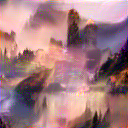
\includegraphics[width=0.45\textwidth]{img/jose-converted.png}
        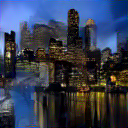
\includegraphics[width=0.45\textwidth]{img/jose-reverse.png}
        \caption{Convertida y Revertida - José}
        \label{jose-1}
    \end{figure}

    \begin{figure}
        \centering
        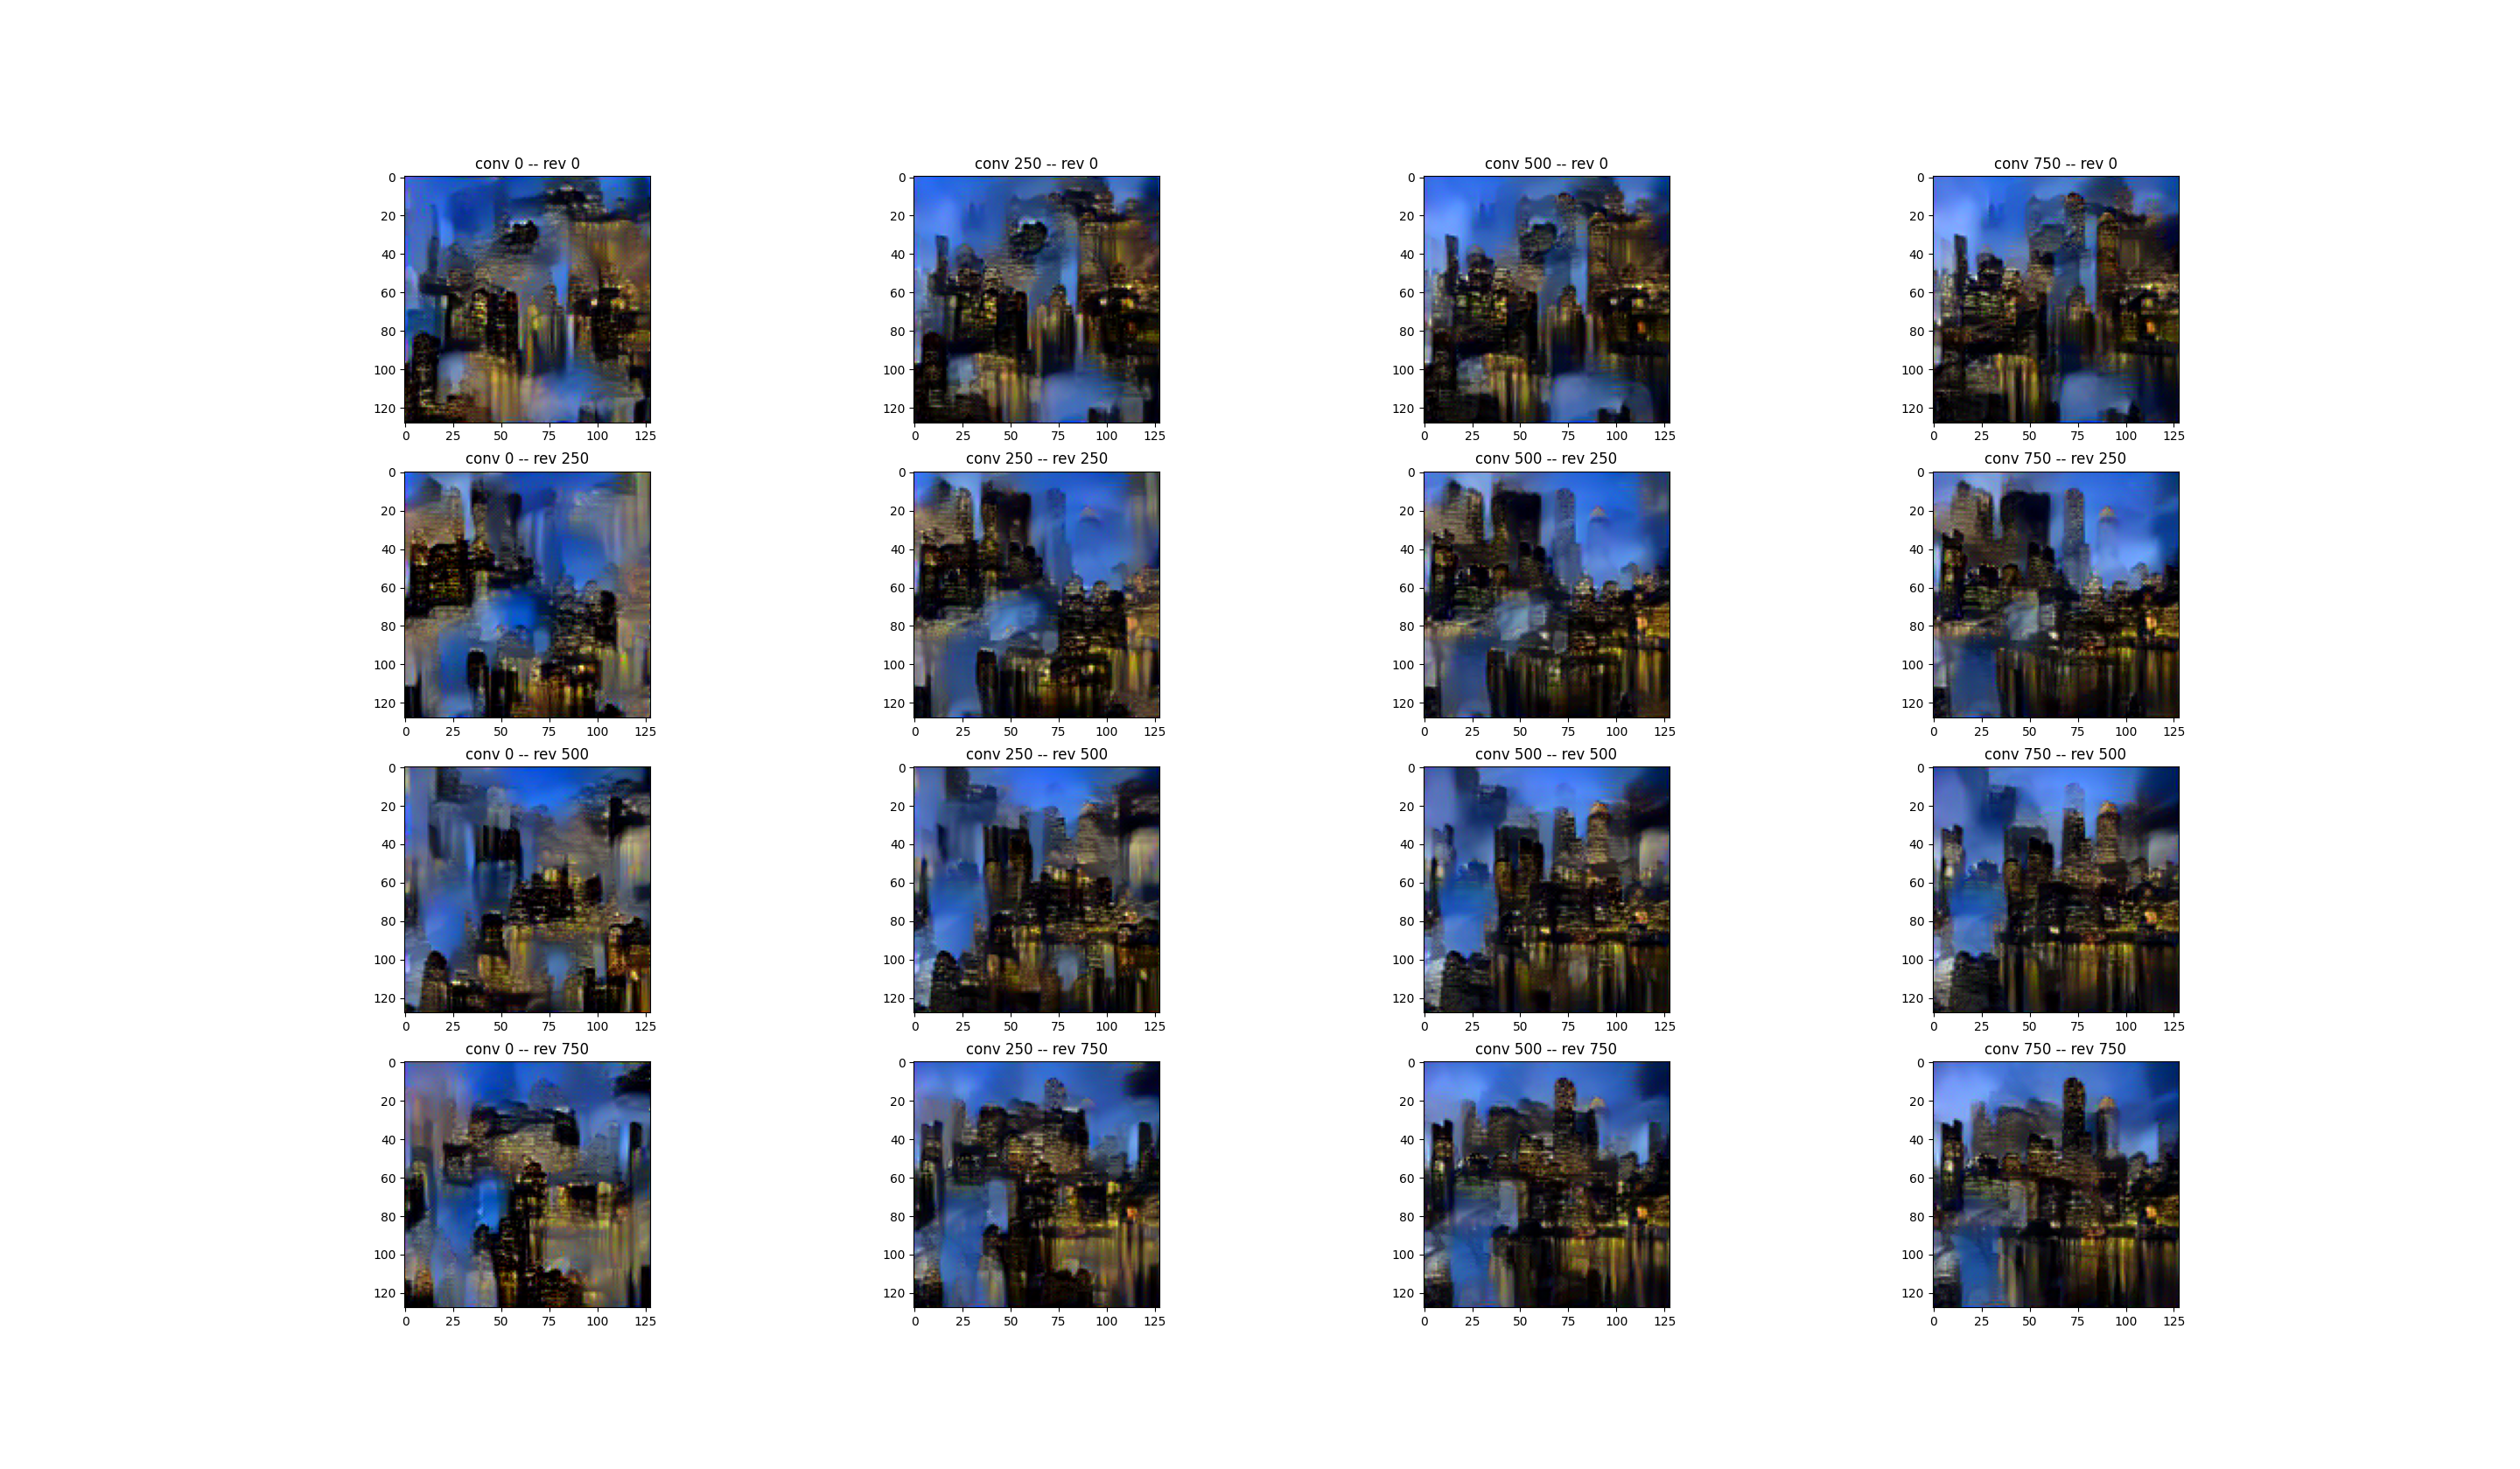
\includegraphics[width=0.6\textwidth]{img/matriz.png}
        \caption{Matriz - José}
        \label{jose-2}
    \end{figure}

    \end{report}


%    % bibliography
%    \label{bibliography}
%    \part{Referencias}
%    \printbibliography
    % \printbibliography[heading=bibintoc,title={Referencias}]  % alternative

    % appendices
%    \begin{appendices}
%        \part{Apéndices}  % optional
%        \section{Mi apéndice}
%        \lipsum[1]
%    \end{appendices}

\end{document}
